% Packages

\documentclass[
	11pt, % Set the default font size, options include: 8pt, 9pt, 10pt, 11pt, 12pt, 14pt, 17pt, 20pt
	%t, % Uncomment to vertically align all slide content to the top of the slide, rather than the default centered
	%aspectratio=169, % Uncomment to set the aspect ratio to a 16:9 ratio which matches the aspect ratio of 1080p and 4K screens and projectors
]{beamer}
\setcounter{tocdepth}{1}
\usepackage{graphicx}
\usepackage[export]{adjustbox}
\graphicspath{{Images/}{./}} % Specifies where to look for included images (trailing slash required)
\usepackage{tikz}
\newenvironment{amatrix}[1]{
    \left[\begin{array}{@{}*{#1}{c}|c@{}}
}{%
    \end{array}\right]
}

\usepackage{booktabs} % Allows the use of \toprule, \midrule and \bottomrule for better rules in tables
\usepackage{pgfplots}
\usepackage{tikz}
\pgfplotsset{width=6cm, compat=newest, every tick label/.append style={scale=0.5}}
\usepackage{amsmath}
\usepackage{blkarray}% http://ctan.org/pkg/blkarray
\newcommand{\matindex}[1]{\mbox{\scriptsize#1}}% Matrix index

% Theme
\usetheme{Madrid}

% Font
\usefonttheme{serif}
\usepackage{newtxtext,newtxmath}
\usepackage[default]{lato}

% Inner theme
\useinnertheme{circles}

% Information
\title{Graph theory}
\author{Kin Hei Wong}
\date{\today}
%%%%%%%%%%%%%%%%%%%%%%%%%%%%%%%%%%%%%%%%%%%%%%%%%%%%%%%%%%
\begin{document}

% Title slide
\begin{frame}
    \titlepage
\end{frame}

% Table of Content
\begin{frame}
    \frametitle{Presentation overview}
    \tableofcontents
\end{frame}
%%%%%%%%%%%%%%%%%%%%%%%%%%%%%%%%%%%%%%%%%%%%%%%%%%%%%%%%%%%
% Body slides

\begin{frame}{Heads Up!}
    \begin{center}
        
\includegraphics[width=10cm]{Proofs.jpg}
    \end{center}
\end{frame}

\section{12A: Graphs and adjacency matrices}
\begin{frame}
    \frametitle{12A}
    \begin{center}
        \title{Graphs and adjacency matrices}
        \maketitle
    \end{center}
\end{frame}

\begin{frame}{What is a graph?}
    \begin{block}{Definition}
        Let there exists a graph G, it consists of:\\
        \begin{enumerate}
            \item a finite non-empty set of elements called vertices
            \item a finite set of elements called edges
            \item an edge-endpoint function that indicates the endpoints of each edge - this function
            maps each edge to a set of either one or two vertices.
        \end{enumerate}
    \end{block}
    \bigskip
    Vertex(Vertices) - Points\\
    Edge - Lines between vertices\\
\end{frame}

\begin{frame}{Matrix representation - adjacency matrix}
    \begin{center}
        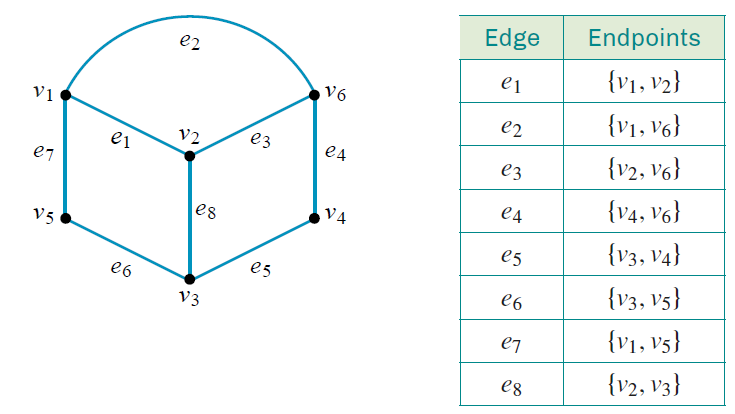
\includegraphics[width = 6cm]{Graph1.png}\\
    \end{center}
    \[
        A = 
        \begin{blockarray}{ccccccc}
            & v_1 & v_2 & v_3 & v_4 & v_5 & v_6 &\\
            \begin{block}{c[cccccc]}
                v_1 & 0 & 1 & 0 & 0 & 1 & 1\\
                v_2 & 1 & 0 & 1 & 0 & 0 & 1\\
                v_3 & 0 & 1 & 0 & 1 & 1 & 0\\
                v_4 & 0 & 0 & 1 & 0 & 0 & 1\\
                v_5 & 1 & 0 & 1 & 0 & 0 & 0\\
                v_6 & 1 & 1 & 0 & 1 & 0 & 0\\ 
            \end{block}
        \end{blockarray}
    \]
\end{frame}

\begin{frame}{Matrix representation - adjacency matrix}
    \begin{center}
        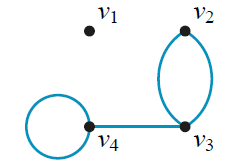
\includegraphics[width = 3cm]{Graph2.png}\\
    \end{center}
    \[
        \begin{blockarray}{ccccc}
            & v_1 & v_2 & v_3 & v_4\\
            \begin{block}{c[cccc]}
                v_1 & 0 & 0 & 0 & 0\\
                v_2 & 0 & 0 & 2 & 0\\
                v_3 & 0 & 2 & 0 & 1\\
                v_4 & 0 & 0 & 1 & 1\\
            \end{block}
        \end{blockarray}
    \]
\end{frame}

\begin{frame}[t]
    \frametitle{Example}
    The following graph represents three houses, A, B and C, that are each connected to
    three utilities, gas (G), water (W) and electricity (E). Construct the adjacency matrix for
    this graph.\\
    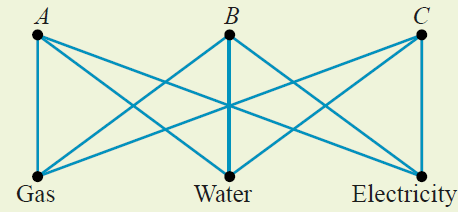
\includegraphics[width = 4cm]{Graph3.png}\\
\end{frame}

\begin{frame}{Different pattern(s)}
    \begin{center}
        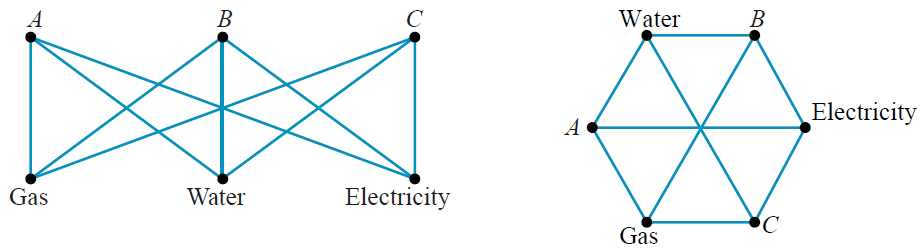
\includegraphics[width = 7cm]{Graph4.png}\\
    \end{center}
\end{frame}

\begin{frame}{Isomorphism}
    \begin{block}{Definition}
        There exists Graph H and G if and only if graph H can be obtained from graph G by simply relabelling its vertices.
        \begin{center}
            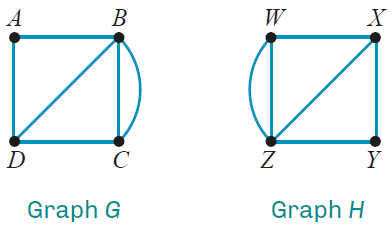
\includegraphics[width = 4cm]{Graph5.png}
        \end{center}
    \end{block}
    By relabelling, we can see the relations of:\\
    \[
        A \leftrightarrow Y, \quad B \leftrightarrow Z, \quad C \leftrightarrow W, \quad D \leftrightarrow X
    \]
\end{frame}

\begin{frame}[t]
    \frametitle{Example}
    Give three reasons why the two graphs shown on the right could not possibly be isomorphic.\\
    \begin{center}
        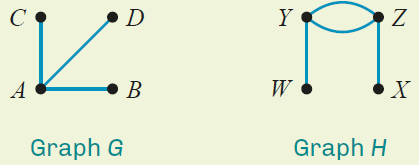
\includegraphics[width = 4cm]{Graph6.png}
    \end{center}
    \begin{block}{Possible solutions:}
        \begin{enumerate}
            \item Graph G does not have multiple edges, while graph H has multiple edges.
            \item Graph G has three edges, while graph H has four edges.
            \item Graph G has one vertex where three edges meet, while graph H has two such vertices.
        \end{enumerate}
    \end{block}
\end{frame}

\begin{frame}{Degree of a vertex}
    \begin{block}{Definition}
        Let $v$ be a vertex of graph G. The degree of $v$ (deg($v$))= number of edges that have vertex $v$ as an endpoint.\\
        Each edge with a loop counts twice.
    \end{block}
    \begin{center}
        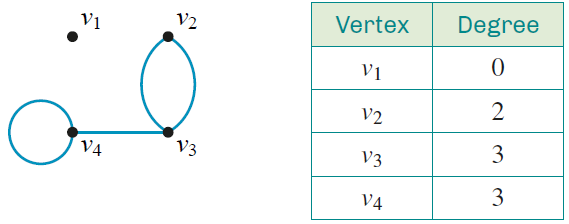
\includegraphics[width = 7cm]{Graph7.png}
    \end{center}
\end{frame}

\begin{frame}[t]
    \frametitle{Handshaking Lemma}
    Note: Lemma is one of a smaller proof to prove on a larger theorem when combined together.\\
    \begin{block}{Handshaking Lemma}
        The total degree of any graph is equal to twice the number of edges of the graph.
    \end{block}
    Proof:\\
    
\end{frame}
\begin{frame}{Handshaking Lemma}
\end{frame}

\begin{frame}{Catogarising Graphs}
    \begin{block}{Simple Graph}
        A graph with no loops or multiple edges.\\
        \begin{center}
            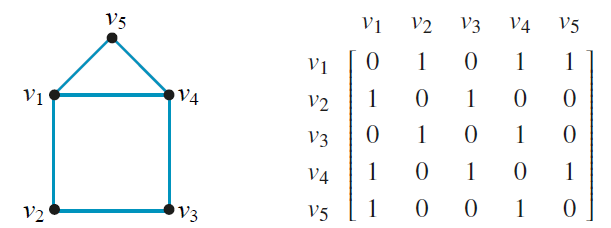
\includegraphics[width = 8cm]{Graph8.png}
        \end{center}
    \end{block}
\end{frame}

\begin{frame}{Catogarising Graphs}
    \begin{block}{Subgraph}
        A graph with no loops or multiple edges.\\
        \begin{center}
            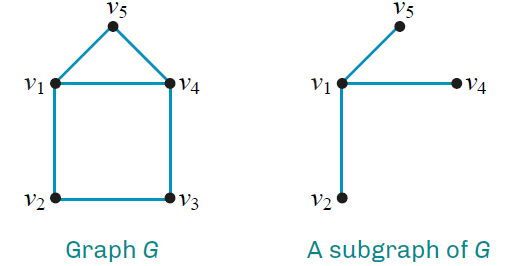
\includegraphics[width = 8cm]{Graph9.png}
        \end{center}
    \end{block}
\end{frame}

\begin{frame}{Exercise 12A}
\end{frame}
%%%%%%%%%%%%%%%%%%%%%%%%%%%%%%%%%%%%%%%%%%%%%%%%%%%%%%%%%%%%%

\section{12B: Euler circuits}
\begin{frame}
    \frametitle{12B}
    \begin{center}
        \title{Euler circuits}
        \maketitle
    \end{center}
\end{frame}

\begin{frame}{Before we go to Euler circuit}
    Let's understand what are walks in graph!
    \begin{block}{Walks in graphs}
        A walk in a graph is an alternating sequence of vertices and edges
        $v_1, e_1, v_2, e_2,\ldots , v_{n-1}, e_{n-1}, v_n$\\
        where the edge $e_i$ joins the vertices $v_i$ and $v_{i+1}$.\\
        \bigskip
        If each pair of adjacent vertices in a walk is joined by only one edge, then the walk can be described by the sequence of vertices $v_1, v_2,\ldots,v_n$.\\
        \begin{center}
            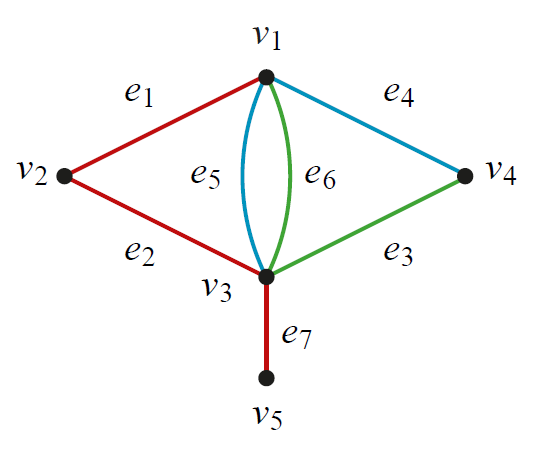
\includegraphics[width = 4.25cm]{Walk.png}
        \end{center}
    \end{block}
\end{frame}

\begin{frame}{Connect vs disconnect graphs}
    \begin{center}
        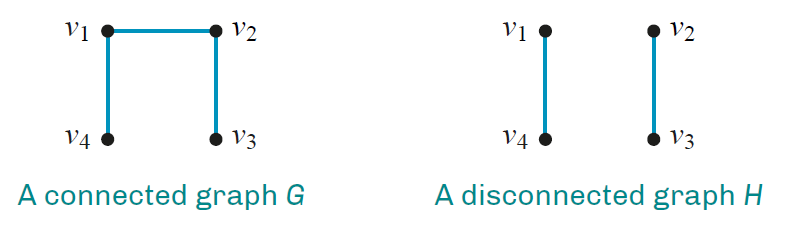
\includegraphics[width = 12cm]{Connect.png}
    \end{center}
\end{frame}

\begin{frame}{Euler trail}
    A trail is a walk in a graph that does not use the same edge more than once. 
    \begin{block}{Euler trail}
       - Uses every edge exactly once\\
       - Some vertices may be visited more than once
        \begin{center}
            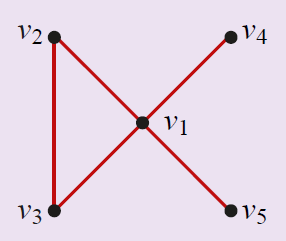
\includegraphics[width = 4cm]{Trail.png}
        \end{center}
        What is the walk?:
    \end{block}
\end{frame}

\begin{frame}{Euler circuit}
    \begin{block}{Euler circuit}
        - uses every edge exactly once\\
        - Starts and ends at the same vertex\\
        \begin{center}
            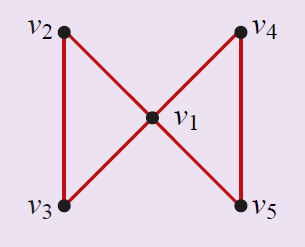
\includegraphics[width = 4cm]{E_circuit.png}
        \end{center}
        What is the walk?:
    \end{block}
\end{frame}

\begin{frame}[t]
    \frametitle{Euler circuit}
    \begin{block}{Theorem}
        A connected graph has an Euler circuit if and only if the degree of every vertex is even.
    \end{block}
    Proof:
\end{frame}
\begin{frame}{Euler circuit}
\end{frame}

\begin{frame}[t]
    \frametitle{Example}
    For each of the following graphs, name an Euler circuit if one exists:
    \begin{center}
        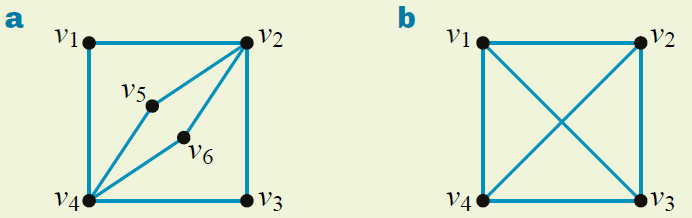
\includegraphics[width = 6cm]{Graph10.png}
    \end{center}
\end{frame}

\begin{frame}[t]
    \frametitle{Euler trail}
    \begin{block}{Theorem}
        A connected graph has an Euler trail if and only if one of the following holds:\\
        \begin{enumerate}
            \item every vertex has even degree
            \item exactly two vertices have odd degree.
        \end{enumerate}
    \end{block}
    Proof:
\end{frame}
\begin{frame}{Euler trail}
\end{frame}

\begin{frame}[t]
    \frametitle{Example}
    For each of the following graphs, name an Euler circuit if one exists:
    \begin{center}
        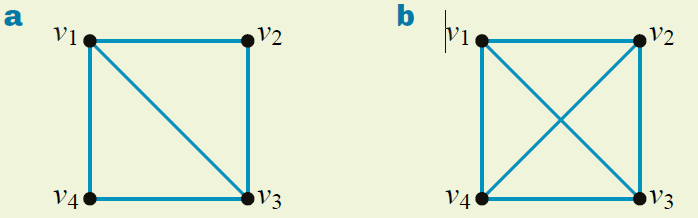
\includegraphics[width = 6cm]{Graph11.png}
    \end{center}
\end{frame}

\begin{frame}{Fleury's algorithm}
    In the real world, there can be many vertices. Hence, we can't just do trial and error. Now Fleury's algorithm comes in handy!\\
    \begin{block}{}
        To find an Euler trail in a connected graph such that every vertex has even degree or exactly two vertices have odd degree:
        \begin{enumerate}
            \item If there are two vertices of odd degree, then start from one of them. Otherwise,
            start from any vertex.
            \item Move from the current vertex across an edge to an adjacent vertex. Always
            choose a non-bridge edge unless there is no alternative.
            \item Delete the edge that you have just traversed.
            \item Repeat from Step 2 until there are no edges left.
        \end{enumerate}
        \begin{center}
            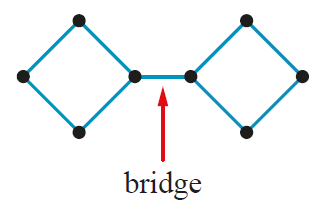
\includegraphics[width = 3cm]{Bridge.png}
        \end{center}
    \end{block}
\end{frame}

\begin{frame}{Try this one}
    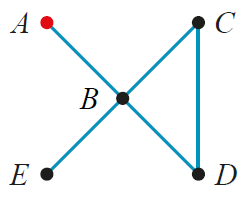
\includegraphics[width = 3cm]{Graph12.png}
\end{frame}

\begin{frame}{Exercise 12B}
\end{frame}
%%%%%%%%%%%%%%%%%%%%%%%%%%%%%%%%%%%%%%%%%%%%%%%%%%%%%%%%%%%%%

\section{12C: Hamiltonian cycles}
\begin{frame}
    \frametitle{12C}
    \begin{center}
        \title{Hamiltonian cycles}
        \maketitle
    \end{center}
\end{frame}

\begin{frame}{Hamiltonian path}
    Path - a walk in graph that does not repeat any vertices (also edges)\\
    \begin{block}{Hamiltonian path}
        - a walk in a graph that visits every vertex exactly once
        \begin{center}
            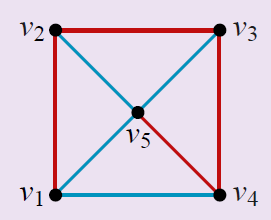
\includegraphics[width = 4cm]{Hamilton.png}
        \end{center}
        What is the walk?:
    \end{block}
\end{frame}

\begin{frame}{Hamiltonian path}
    Cycle - walk that starts and end at the same vertex, also does not repeat any vertex or edges\\
    \begin{block}{Hamiltonian path}
        - walk that starts and ends at the same vertex and visits every other vertex exactly once
        \begin{center}
            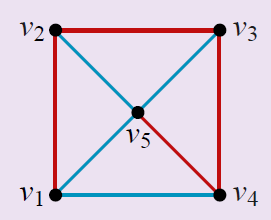
\includegraphics[width = 4cm]{Hamilton.png}
        \end{center}
        What is the walk?:
    \end{block}
    Note: Hamilton path or cycle, some edges may not be used
\end{frame}

\begin{frame}[t]
    \frametitle{Example}
    Eight towns are represented by the vertices $v_1, v_2, \ldots, v_8$. The
roads that connect these towns are represented as edges. Starting
and ending at $v_1$, how can a salesperson visit every town exactly
once?
    \begin{center}
        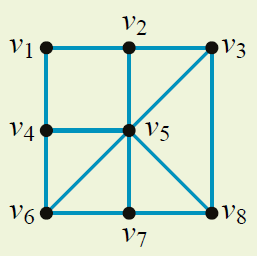
\includegraphics[width = 4cm]{Graph13.png}
    \end{center}
\end{frame}

\begin{frame}{Difference between Euler and Hamiltonian}
    \begin{enumerate}
        \item \alert{E}uler are defined in terms of \alert{E}dges
        \item If a graph has Euler, then no Hamiltonian
        \item If a graph has Hamiltonian, then no Euler
    \end{enumerate}
    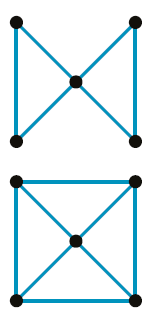
\includegraphics[width = 3cm]{Graph14.png}
\end{frame}

\begin{frame}{Exercise 12C}
\end{frame}
%%%%%%%%%%%%%%%%%%%%%%%%%%%%%%%%%%%%%%%%%%%%%%%%%%%%%%%%%%%%%

\section{12D: Using matrix powers to count walks in graphs}
\begin{frame}
    \frametitle{12D}
    \begin{center}
        \title{Using matrix powers to count walks in graphs}
        \maketitle
    \end{center}
\end{frame}

\begin{frame}[t]
    \frametitle{Length of a walk}
    \begin{block}{Definition}
        Length of a walk in a graph is the number of edges in the walk.\\
        If you use the same edge more than once, then you must count that edge more than once
    \end{block}
    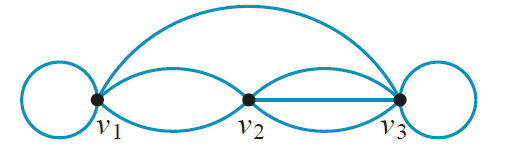
\includegraphics[width = 5cm]{Length.png}\\
    How does length of 1 look like?\\
    $v_1 \rightarrow v_3$\\
    $v_2 \rightarrow v_3$\\
    $v_1 \rightarrow v_2$\\
\end{frame}

\begin{frame}[t]
    \frametitle{Walk of length 2}
    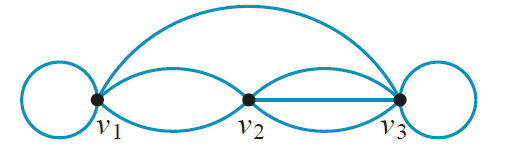
\includegraphics[width = 5cm]{Length.png}\\
    What is the number of walks of length 2 from $v_1 \rightarrow v_3$
    Case 1: $v_1 \rightarrow v_1 \rightarrow v_3$\\
    Case 2: $v_1 \rightarrow v_2 \rightarrow v_3$\\
    Case 2: $v_1 \rightarrow v_3 \rightarrow v_3$\\
    
\end{frame}

\begin{frame}{Matrix power comes in handy!}
    Walk of length 1:
    \[A =
        \begin{blockarray}{cccc}
            & v_1 & v_2 & v_3\\
            \begin{block}{c[ccc]}
                v_1 & 1 & 2 & 1\\
                v_2 & 2 & 0 & 3\\
                v_3 & 1 & 3 & 1\\
            \end{block}
        \end{blockarray}
    \]
    \bigskip
    Walk of length 2:
\end{frame}

\begin{frame}[t]
    \frametitle{Example}
    Note: It is helpful to define $A^0 = I$, where $I$ is the identity matrix. We can then also consider
    walks of length 0. We say that there is one walk of length 0 from any vertex to itself.\\
    \begin{block}{}
        Find the number of walks of length 3 from vertex v1 to vertex v3 in the graph shown.\\
    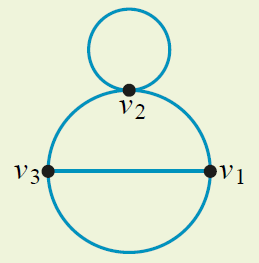
\includegraphics[width = 3cm]{Graph15.png}\\
    \end{block}
\end{frame}

\begin{frame}{Exercise 12D}
\end{frame}
%%%%%%%%%%%%%%%%%%%%%%%%%%%%%%%%%%%%%%%%%%%%%%%%%%%%%%%%%%%%%

\section{12E: Regular, cycle, comple and bipartite graphs}
\begin{frame}
    \frametitle{12E}
    \begin{center}
        \title{Regular, cycle, comple and bipartite graphs}
        \maketitle
    \end{center}
\end{frame}

\begin{frame}[t]
    \frametitle{Regular graphs}
    A graph is said to be regular if all its vertices have the same degree.\\
    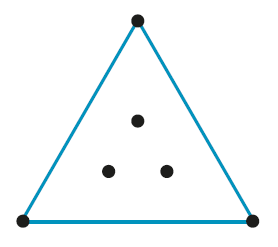
\includegraphics[width = 2cm]{Regular.png}\\
    \begin{block}{Theorem}
        If $G$ is a regular graph with $n$ vertices of degree $r$, then $G$ has $\frac{nr}{2}$ edges.
    \end{block}
    Proof:
\end{frame}

\begin{frame}[t]
    \frametitle{Cycle graphs}
    A cycle graph is consisting of a single cycle of vertices and edges. For $n\geq 3$, the cycle graph with $n$ vertices is denoted by $C_n$.\\
    \begin{center}
        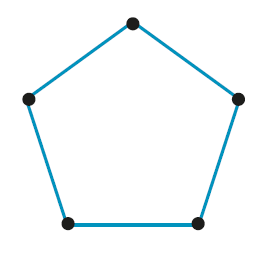
\includegraphics[width = 2cm]{Cycle.png}\\
    \end{center}

    Every cycle graph $C_n$ is regular, since each vertex has degree 2. The cycle graph $C_5$ is shown above.
\end{frame}

\begin{frame}[t]
    \frametitle{Complete graphs}
    A complete graph is a simple graph with 1 edge joining each pair of distinct vertices. With $n$ vertices, it is denoted by $K_n$.\\
    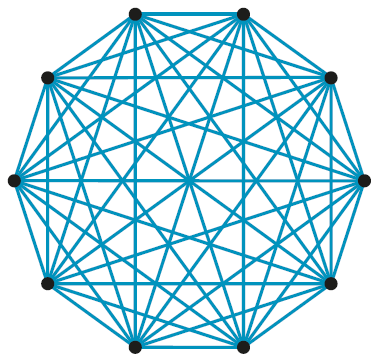
\includegraphics[width = 2cm]{Complete.png}\\
    It is $K_10$ above! The graph $K_n$ is regular, since each vertex has degree $n-1$. Adjancency matrix of $K_n$ has 1s in all poitions (except for main diagonal being 0s.)\\
    \begin{block}{Theorem}
        The complete graph $K_n$ has $\frac{n(n-1)}{2}$ edges.
    \end{block}
    Proof:
\end{frame}

\begin{frame}
\end{frame}

\begin{frame}{Complement of simple graph}
    \begin{block}{Complement of simple graph}
        If $G$ is a simple graph, complement $G$ is $\bar{G}$:\\
        \begin{enumerate}
            \item $\bar{G}$ and G have the same set of vertices
            \item Two vertices are adjacent in $\bar{G}$ iff the are not adjacent in $G$.
        \end{enumerate}
    \end{block}
    Note: To generate the complement of a simple graph, fill in all the missing edges required to
    form a complete graph and then remove all the edges of the original graph.
\end{frame}

\begin{frame}[t]
    \frametitle{Example}
    \begin{enumerate}
        \item How many edges does the complete graph $K_5$ have?
        \item Draw $K_5$
        \item Draw the cycle graph $C_5$ and draw the complement of $C_5$.
    \end{enumerate}
\end{frame}

\begin{frame}{Bipartite graph}
    A bipartite graph is a graph whose vertcies can be divided into two disjoint subsets $A$ and $B$ such that every edge of the graph joins a vertex in
    $A$ to a vertex in $B$.\\
    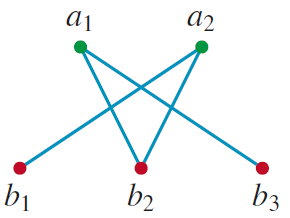
\includegraphics[width = 4cm]{Bipart.png}\\
    Every edge of the graph joins a vertex in $A = {a_1, a_2}$ to a vertex in $B = {b_1, b_2, b_3}$.
\end{frame}

\begin{frame}{Complete bipartite graph}
    A bipartite graph is a simple graph whose vertcies can be divided into two disjoint subsets $A$ and $B$ such that\\
    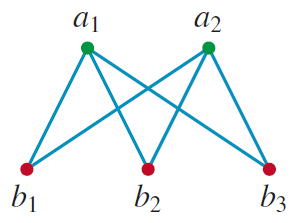
\includegraphics[width = 4cm]{C_bipart.png}\\
    \begin{enumerate}
        \item every edge joins a vertex in $A$ to a vertex in $B$
        \item every vertex in $A$ is joined to every vertex in $B$
    \end{enumerate}
    The complete bipartite graph where $A$ contains $m$ vertices and $B$ contains $n$ vertices is denoted by $K_{m,n}$.
\end{frame}

\begin{frame}[t]
    \frametitle{Example}
    Draw the complete bipartite graph $K_{2,4}$ and give its adjacency matrix.
    
\end{frame}

\begin{frame}[t]
    \frametitle{Example}
    \begin{enumerate}
        \item Show that the cycle graph $C_6$ is a bipartite graph by dividing the set of vertices into two
        suitable disjoint subsets.
        \item Hence show that $C_6$ is a subgraph of $K_{3,3}$.
    \end{enumerate}
    
\end{frame}
\begin{frame}
\end{frame}

\begin{frame}{Exercise 12E}
\end{frame}
%%%%%%%%%%%%%%%%%%%%%%%%%%%%%%%%%%%%%%%%%%%%%%%%%%%%%%%%%%%%%

\section{12F: Trees}
\begin{frame}
    \frametitle{12F}
    \begin{center}
        \title{Trees}
        \maketitle
    \end{center}
\end{frame}

\begin{frame}{Trees}
    \begin{block}{Definition}
        Tree is a connected graph without any cycle
        \begin{center}
            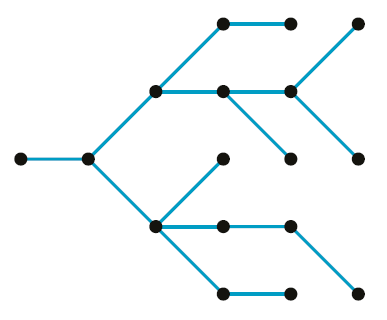
\includegraphics[width = 4cm]{Tree.png}\\
        \end{center}
    \end{block}
    Properties:
    \begin{enumerate}
        \item A tree with $n$ vertices has $n - 1$ edges.
        \item In any tree, there is exactly one path between each pair of distinct vertices.
        \item Every tree is a bipartite graph.
    \end{enumerate}
\end{frame}

\begin{frame}[t]
    \frametitle{Example}
    Draw the three trees with five vertices.
\end{frame}

\begin{frame}[t]
    \frametitle{Example}
    Show that this tree is a bipartite graph by dividing its vertices into two suitable disjoint subsets.\\
    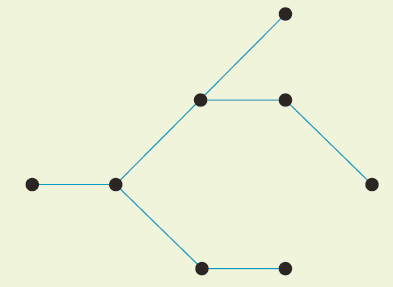
\includegraphics[width=6cm]{Tree2.png}
\end{frame}

\begin{frame}{Spanning trees}
    \begin{block}{Definition}
        Let $G$ be a connected graph. Spanning tree of $G$ is a subgraph of $G$ that is a tree with same set of vertices of G.
        \begin{center}
            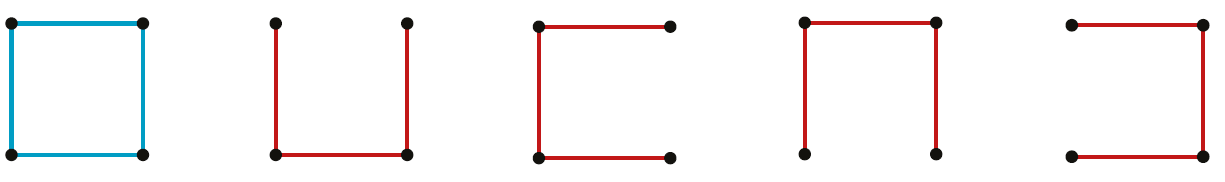
\includegraphics[width = 8cm]{Span.png}\\
        \end{center}
    \end{block}
    \begin{block}{Theorem}
        Every connected graph has a spanning tree.
    \end{block}
\end{frame}

\begin{frame}{Algorithm for finding a spanning tree}
    \begin{enumerate}
        \item If the graph has no cycles, then stop.
        \item Choose any edge that belongs to a cycle, and delete the chosen edge.
        \item Repeat from Step 1
    \end{enumerate}
\end{frame}

\begin{frame}[t]
    \frametitle{Example}
    Find a spanning tree for the complete graph $K_5$.    
\end{frame}
\begin{frame}
\end{frame}

\begin{frame}{Exercise 12F}
\end{frame}
%%%%%%%%%%%%%%%%%%%%%%%%%%%%%%%%%%%%%%%%%%%%%%%%%%%%%%%%%%%%%

\section{12G: Euler's formula and the Platonic solids}
\begin{frame}
    \frametitle{12G}
    \begin{center}
        \title{Euler's formula and the Platonic solids}
        \maketitle
    \end{center}
\end{frame}

\begin{frame}{Planar graphs}
    \begin{block}{Definition}
        A graph G is a planar graph if:\\
        \begin{enumerate}
            \item Only edges intersect at their endpoints
            \item Edges does not interset with each other
        \end{enumerate}
        This is known as plane drawing of G.\\
        \begin{center}
            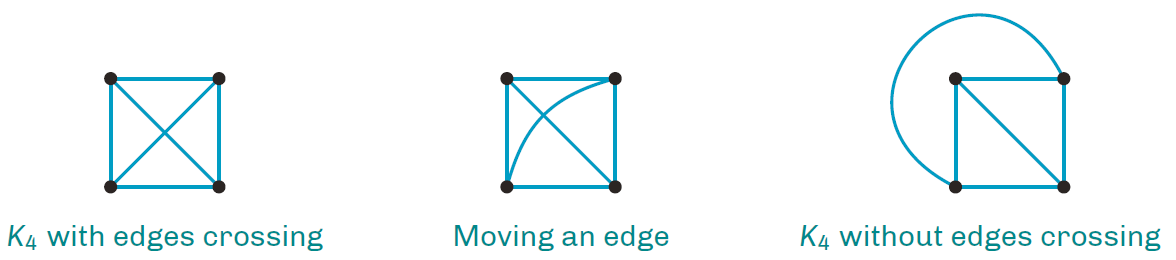
\includegraphics[width = 8cm]{Planar.png}\\
        \end{center}
    \end{block}
\end{frame}

\begin{frame}{This is not Planar graph!}
    You can give it a go to see if it can be changed to planar, but there is proof that it is not planar graph!\\
    \begin{center}
        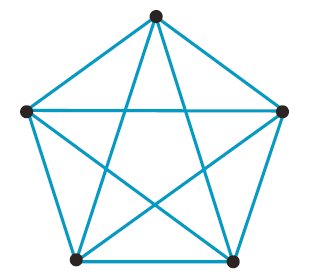
\includegraphics[width = 6cm]{N_planar.png}\\
    \end{center}
\end{frame}

\begin{frame}[t]
    \frametitle{Subgraphs of planar graphs}
    \begin{block}{Theorem}
        Any subgraph of a planar graph is also planar
    \end{block}
    Proof:
\end{frame}

\begin{frame}{Euler's formula}
    \begin{block}{Faces of a planar graph}
        If $G$ is a planar graph:
        \begin{enumerate}
            \item Faces - any plane drawing of $G$ divides the plane into regions
            \item Bounded faces - faces that are bordered by edges
            \item Unbounded face - face that is not bordered by edges
        \end{enumerate}
    \end{block}
    Task: Identify which are bounded and unbounded.
    \begin{center}
        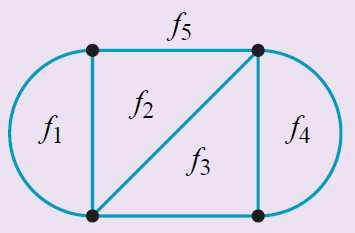
\includegraphics[width = 6cm]{Bounded.png}\\
    \end{center}
\end{frame}

\begin{frame}[t]
    \frametitle{Euler's formula}
    \begin{block}{Theorem}
        If $G$ is a connected planar graph with $v$ vertices, $e$ edges and $f$ faces, then:\\
    $v-e+f=2$
    \end{block}
    Proof:
\end{frame}
\begin{frame}
\end{frame}


\begin{frame}[t]
    \frametitle{Example}
    Verify Euler’s formula for the planar graph shown.
    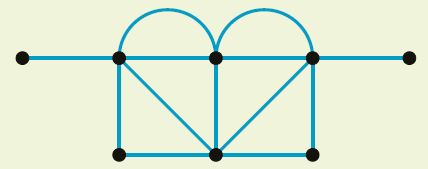
\includegraphics[width=6cm]{Graph16.png}
\end{frame}

\begin{frame}[t]
    \frametitle{Edges of planar graphs}
    \begin{block}{Theorem}
        Let $G$ be a connected simple graph with $v$ vertices and $e$ edges, where $v \geq 3$. If the
        graph $G$ is planar, then $e \leq 3v - 6$.
    \end{block}
    Proof:
\end{frame}
\begin{frame}
\end{frame}

\begin{frame}[t]
    \frametitle{Example}
    A connected simple graph has 6 vertices and 14 edges. Show that this graph is not planar.
\end{frame}

\begin{frame}{Polyhedral graphs}
    A polyheadral is a three-dimensional solid formed from a collection of polygons joined along their edges.\\
    \begin{block}{}
        Every convex polyhedron can be drawn as a connected planar graph.
    \end{block}
    \begin{center}
        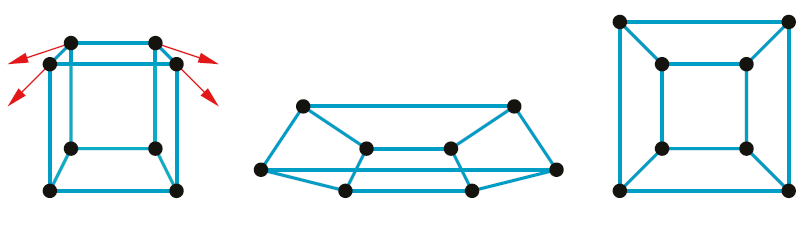
\includegraphics[width=6cm]{Poly1.png}
    \end{center}
\end{frame}

\begin{frame}[t]
    \frametitle{Example}
    A pentagonal prism is shown.
    \begin{enumerate}
        \item Give a plane drawing of the graph that represents the
        pentagonal prism.
        \item Verify Euler’s formula for this graph.
    \end{enumerate}
    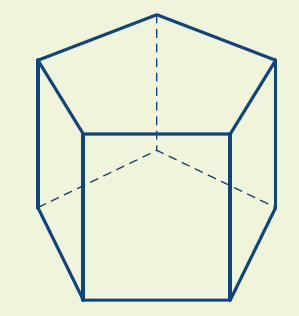
\includegraphics[width=4cm]{Poly2.png}
\end{frame}

\begin{frame}{Platonic solid}
    Platonic solid is a convex polyhedron such that:
    \begin{enumerate}
        \item Polygonal faces are all congruent (identical in shape and in size) and regular (all angles and sides are equal)
        \item The same number of faces meet at each vertex
    \end{enumerate}
    \begin{center}
        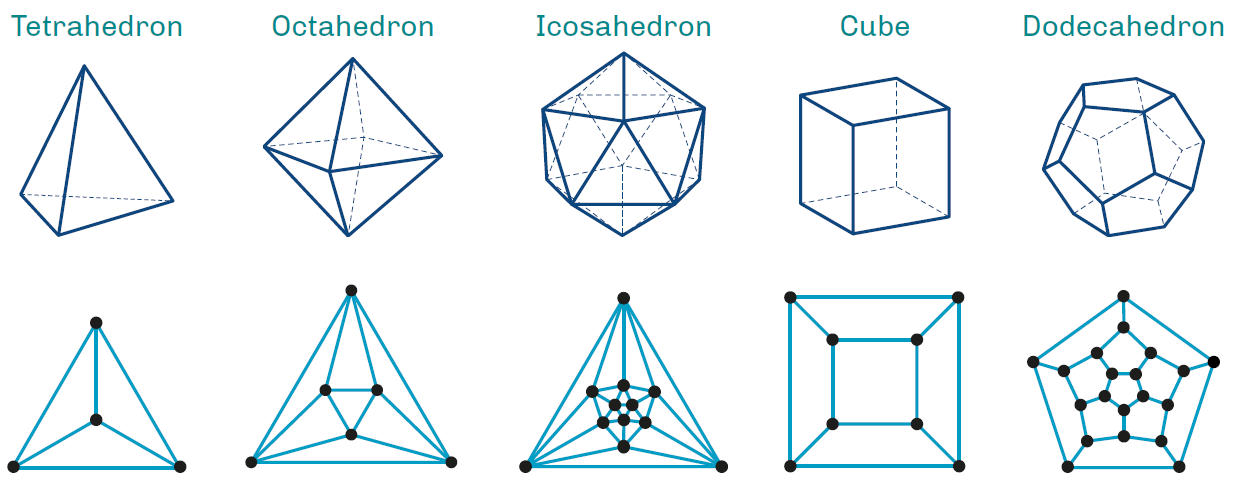
\includegraphics[width=8cm]{Poly3.png}
    \end{center}

\end{frame}

\begin{frame}[t]
    \frametitle{Platonic solid}
    \begin{block}{Theorem}
        There are only five Platonic solids.
    \end{block}
    Proof:
\end{frame}

\begin{frame}{Exercise 12G}
\end{frame}
%%%%%%%%%%%%%%%%%%%%%%%%%%%%%%%%%%%%%%%%%%%%%%%%%%%%%%%%%%%%%

\begin{frame}
    \begin{center}
        
\includegraphics[width=8cm]{Wait.jpg}    
    \end{center}
\end{frame}

\section{12H: When every vertex has even degree}
\begin{frame}
    \frametitle{12H}
    \begin{center}
        \title{When every vertex has even degree}
        \maketitle
    \end{center}
\end{frame}

\begin{frame}[t]
    \frametitle{This is from Section 12B}
    \begin{block}{Theorem - Euler circuits}
        A connected graph has an Euler circuit iff the degree of every vertex is even.
    \end{block}
    We only proved halfway on this theory, we still need to prove if the degree of every vertex is even, then the connected graph has a Euler's circuit.
    \begin{block}{Theorem}
        Let $G$ be a graph in which every vertex has even degree. Then $G$ can be split into cycles,
no two of which have an edge in common.
    \end{block}
    Proof:
\end{frame}
\begin{frame}
\end{frame}
\begin{frame}
\end{frame}

\begin{frame}[t]
    We can now proof the theorem on Euler's circuit\\
    \begin{block}{Theorem}
        A connected graph has an Euler circuit if every vertex has even degree.
    \end{block}
\end{frame}
\begin{frame}
\end{frame}

\begin{frame}{Exercise 12H}
\end{frame}

\begin{frame}
    \begin{center}
        
\includegraphics[width=8cm]{Done.jpg}
    \end{center}
\end{frame}

\end{document}